\documentclass[10pt]{beamer}
\usetheme[outer/progressbar=foot]{metropolis}
\usepackage{booktabs}
%\usepackage[scale=2]{ccicons}
\usepackage{pgfplots}
\usepackage[ngerman]{babel}
\usepackage[utf8]{inputenc}
\usepackage{blindtext}
\usepackage{amsmath}
\usepackage[italicdiff]{physics}
\usepackage[italic]{hepnames}
\usepackage{graphicx}
\usepackage{float}
\usepackage{color}
\usepackage{physics}
\usepackage{tikz}
\usepackage[absolute,overlay]{textpos}
\usepackage[texcoord,grid,gridcolor=red!10,subgridcolor=green!10,gridunit=pt]{eso-pic}

\usepgfplotslibrary{dateplot}


%Frontpage
\title{Calorimetry and Deep Learning}
\date{\today}
\author{Simon Schnake}
\institute{Universität Hamburg}

%Document
\begin{document}
\maketitle
\tikzstyle{every picture}+=[remember picture]
\begin{frame}{Calorimetry in Particle Physics}

\end{frame}

\begin{frame}{Deep Learning}

\end{frame}

\begin{frame}{Simulation Setup}
  \begin{columns}
    \column{0.5\textwidth}
    \begin{textblock*}{150pt}(2pt,55pt)
      \begin{itemize}
      \item Simulation with Geant4\small{}
      \item $e^-$ from 0. to 10 GeV
      \end{itemize}
    \end{textblock*}
    \begin{textblock*}{10pt}(2pt,100pt)
      \begin{tabular}{l|l|l}
        layer  & scint    & absorber \\ \hline
        layer 0      & 9mm     & 40 mm SS\\
        layer 1 - 8  & 3.7mm   & 50.5 mm brass        \\
        layer 9 - 14 & 3.7mm   & 56.5 mm brass         \\
        layer 15     & 3.7 mm  & 75 mm SS \\
        layer 16     & 9mm     &                      
      \end{tabular}
    \end{textblock*}
    \column{0.5\textwidth}
    \begin{figure}[htp]
      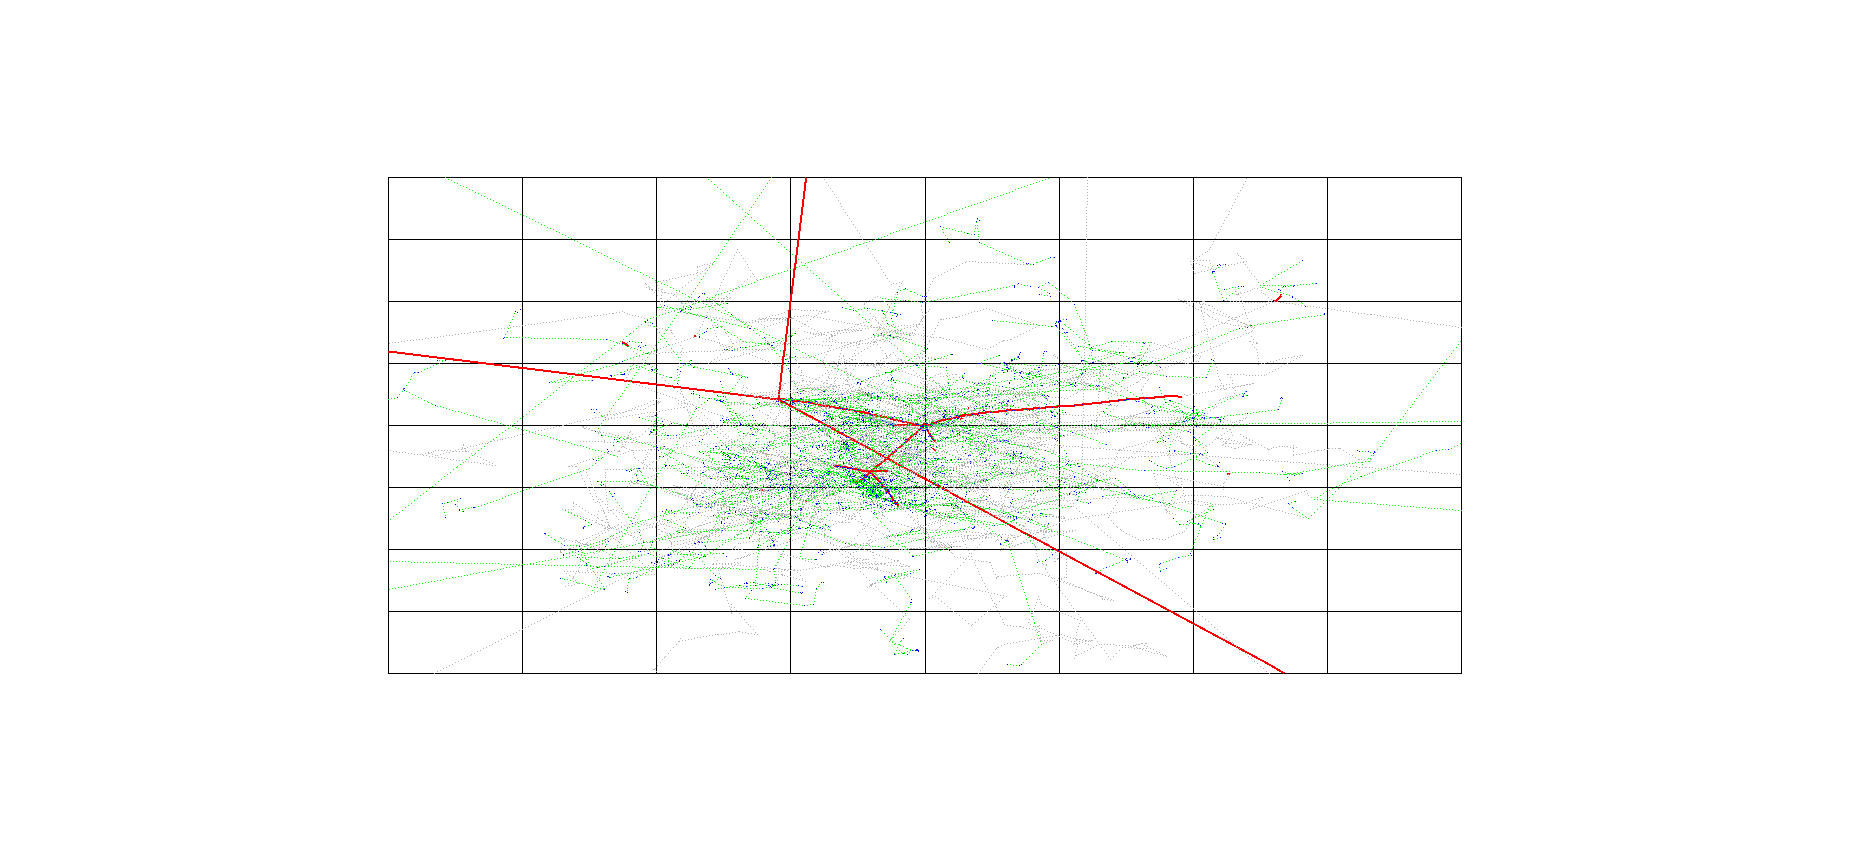
\includegraphics[width=1.1\textwidth]{front.png}\\
      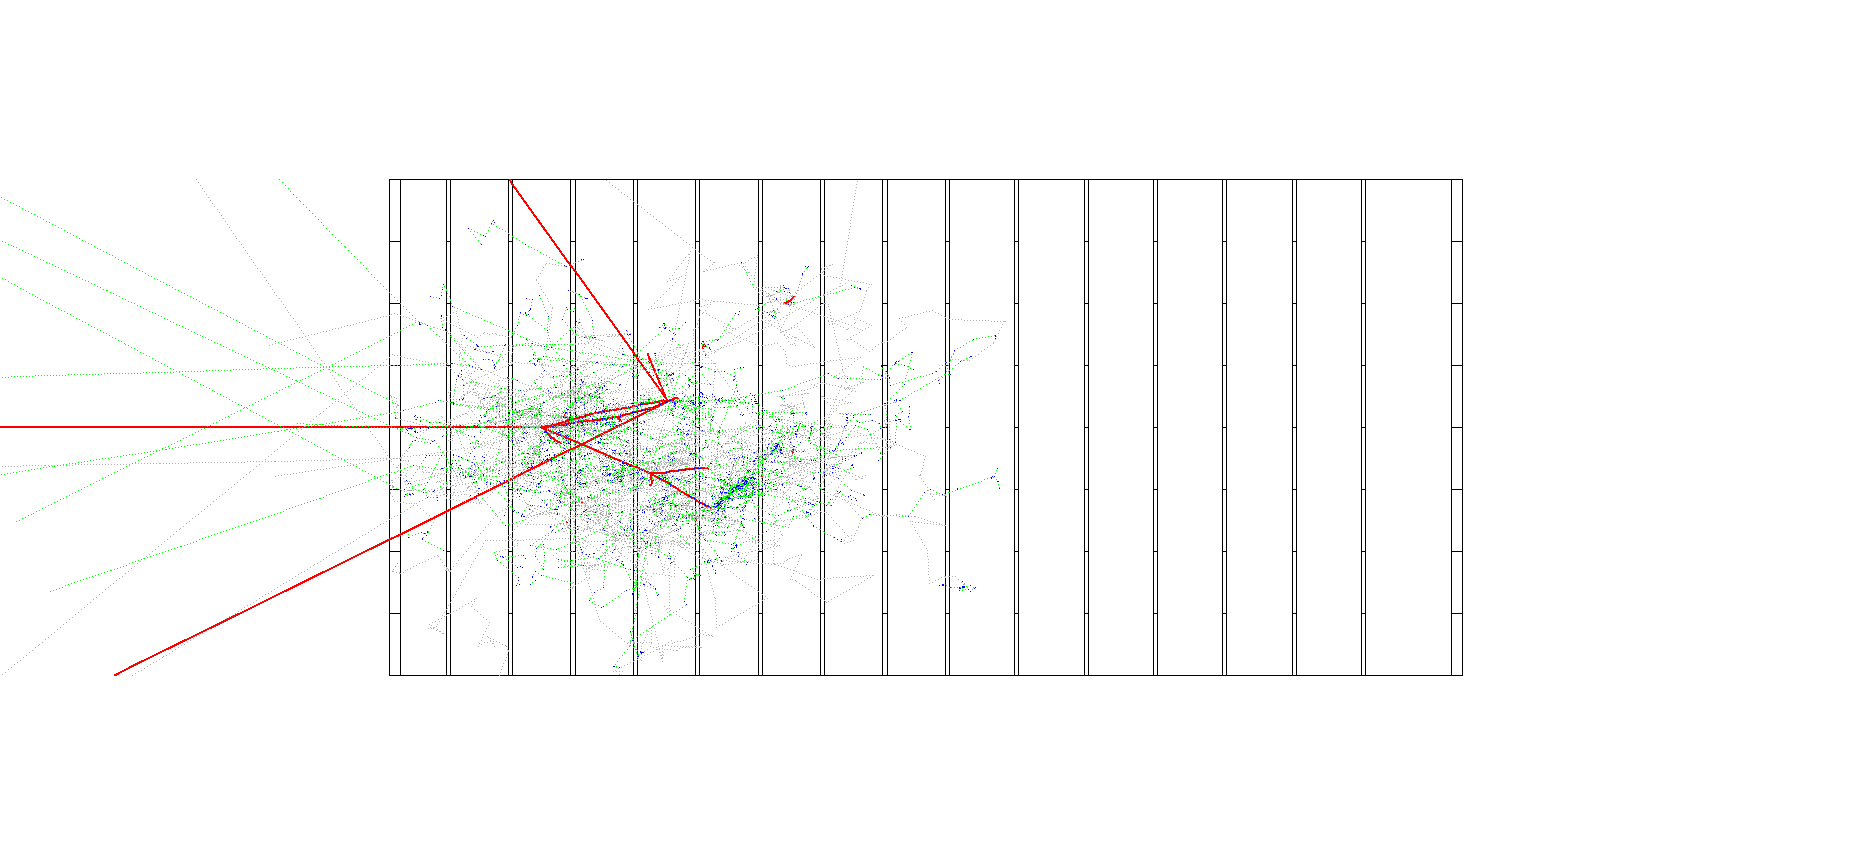
\includegraphics[width=1.1\textwidth]{side.png}
    \end{figure}
  \end{columns}
  \begin{textblock*}{100pt}(250pt,70pt)
    Front view
  \end{textblock*}
  \begin{textblock*}{100pt}(250pt,150pt)
    Side view
  \end{textblock*}
\end{frame}

\begin{frame}{Resulting Data}
  \begin{columns}
    \column{0.5\textwidth}
    \begin{figure}[htp]
      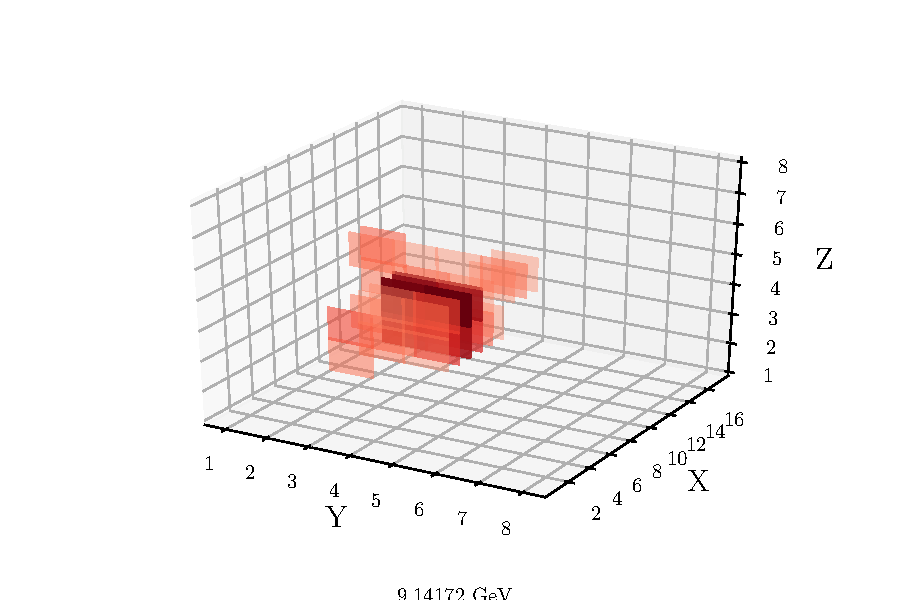
\includegraphics[width=1.1\textwidth]{../data_display.pdf}
    \end{figure}
    \column{0.5\textwidth}
    \begin{figure}[htp]
      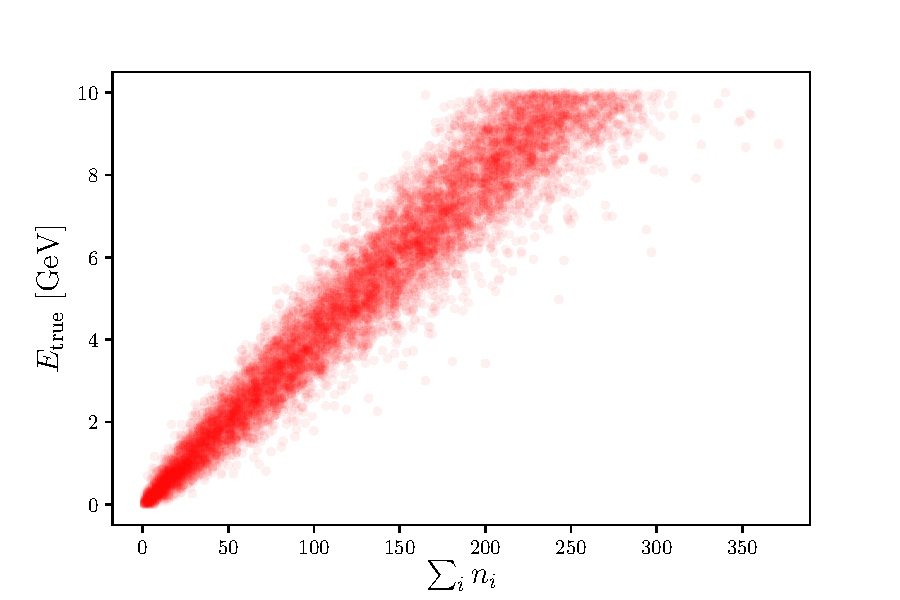
\includegraphics[width=1.1\textwidth]{../e-vs-sum_n.pdf}
    \end{figure}
  \end{columns}
\end{frame}

\begin{frame}{Linear Fit}
    \begin{figure}[htp]
      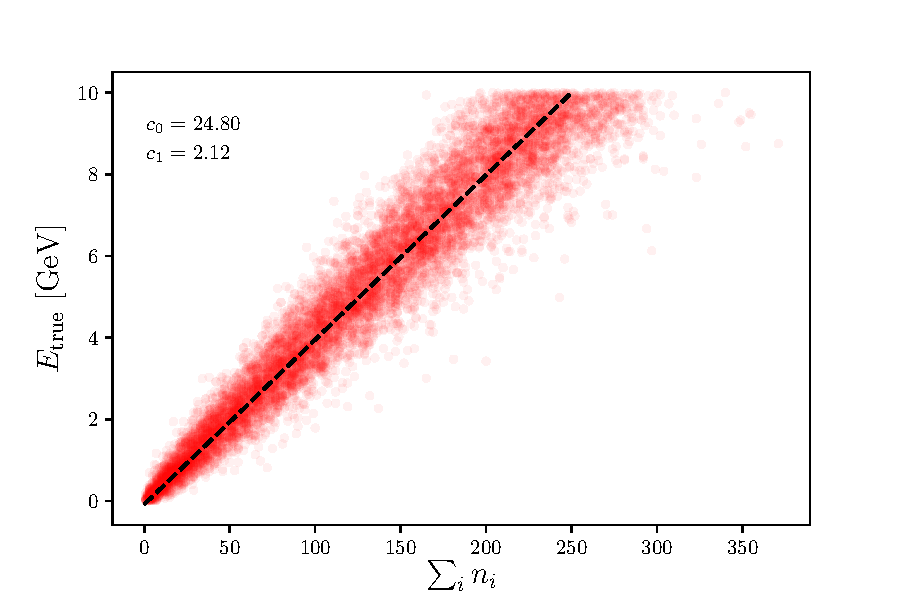
\includegraphics[width=\textwidth]{../e-vs-sum_n_fit.pdf}
    \end{figure}  
\end{frame}

\begin{frame}{First Results of the Neuralnet}
  \begin{columns}
    \column{0.5\textwidth}
    \begin{figure}[htp]
      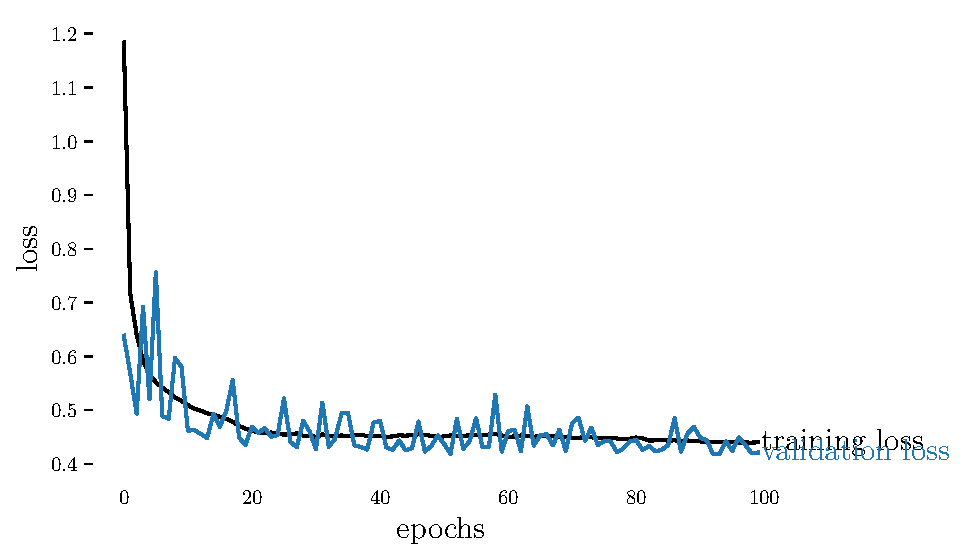
\includegraphics[width=1.1\textwidth]{../loss.pdf}
    \end{figure}
    \column{0.5\textwidth}
    \begin{figure}[htp]
      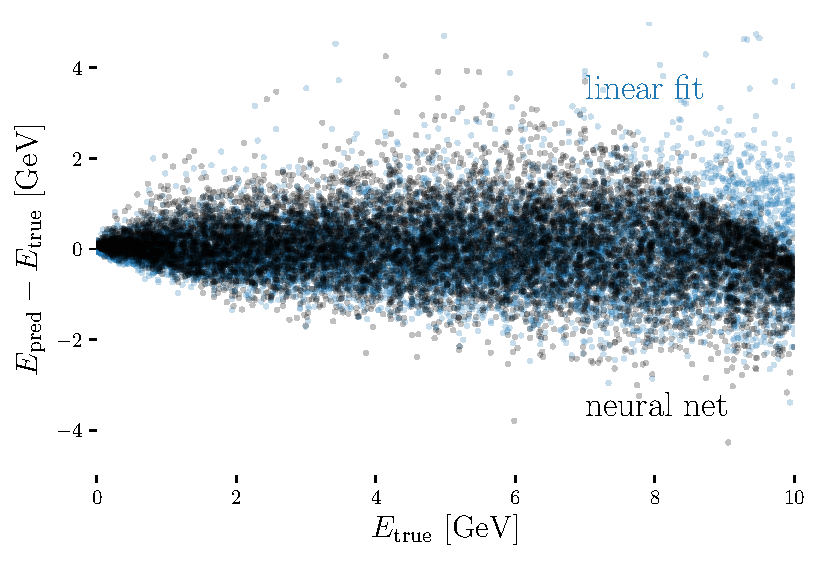
\includegraphics[width=1.1\textwidth]{../first.pdf}
    \end{figure}
  \end{columns}
\end{frame}

\begin{frame}{Data Augmentation}

\end{frame}

\begin{frame}{Maximum Likelihood Loss}

\end{frame}

\begin{frame}{Adversary Training}

\end{frame}

\begin{frame}{Summary}

\end{frame}

\end{document}
